\chapter{Scoops3D.}
\label{chap_Scoops3d}

Scoops3D es una herramienta software disponible por medio de una \emph{Interfaz Gr\'afica de Usuario} (GUI, de las siglas en Ingl\'es de \textit{Graphical User Interface}) para plataformas Microsoft Windows, Mac y Unix. Tambi\'en se puede usar como un conjunto de m\'odulos y funciones en procesos por lotes (i.e. \textit{script}) en el lenguaje computacional Python para ser usado como una clase independiente. Fue desarrollado y es mantenido por el Servicio Geol\'ogico de Estados Unidos (USGS) y tiene como finalidad llevar a cabo a\'nalisis de estabilidad en las laderas a partir de un modelo de elevaci\'on digital (DEM) introducido.\\

Transformando cada p\'ixel del DEM introducido en una columna, Scoops3D analiza autom\'aticamente varias superficies de falla potenciales mediante an\'alisis de equilibro limite.  Como resultado se obtiene un archivo de im\'agen (raster) con los factores de seguridad (indicadores de estabilidad) para la zona estudiada.\\

La capacidad de trabajar sobre zonas que se extienden por miles de kil\'ometros cuadrados a la vez que se tienen en cuenta distintas caracter\'isticas geol\'ogicas, geot\'ecnicas y condiciones variables de saturaci\'on parcial en profundidad, le da a Scoops3D una gran ventaja sobre herramientas computacionales cuyo funcionamiento se limita a perfiles bidimiensionales.
Scoops3D se fundamenta en los m\'etodos de dobelas de Bishop y Fellenius, lo que implica que solamente es aplicable al an\'alisis de superficies de falla de tipo rotacional.

\begin{figure}[H]
\centering
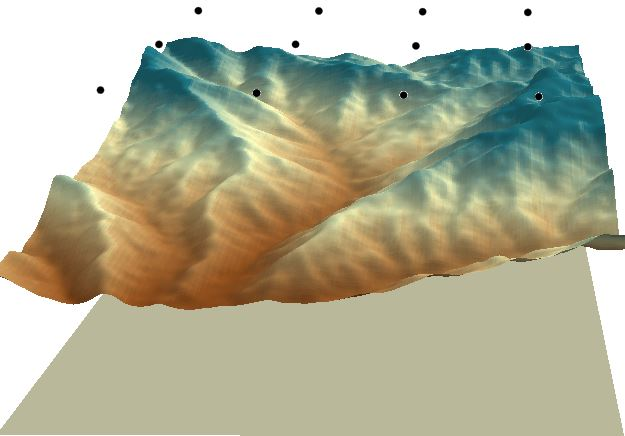
\includegraphics[width=0.8\textwidth]{INTRO.JPG}
\caption{Rejilla de centros de esfera de falla sobre la superficie digital que representa la zona de trabajo. Elaboraci\'on propia.}
\end{figure}
Es importante resaltar que, adem\a's de no estar contemplado entre los alcance ni objetivos de este proyecto, Scoops3D no posee la capacidad de simular el comportamiento de un eventual flujo de lodo o escombros desencadenado por un evento de deslizamiento o falla. 
